\graphicspath{{Chapters/Detector/Figures/}}
\chapter{The ATLAS Detector at the LHC}
\label{chap:Detector}

\section{The Large Hadron Collider}

The Large Hadron Collider (LHC) is a particle accelerator located at CERN, the
European Organisation for Nuclear Research, on the French-Swiss border near
Geneva. The LHC is the world's most powerful particle accelerator, colliding
beams of protons together at centre of mass energies of up to 8 \TeV, with the
aim of better understanding the workings of our Universe. It is installed in a
tunnel of circumference 26.7 km, which previously held the Large
Electron-Positron Collider (LEP), and is between 45 and 170 m below the ground.
The beams are brought to collision at four points around the ring, at each of
which a different experiment is located. The machine is also capable of
colliding heavy ions, providing a complementary heavy-ion physics program.

The design of the LHC is described in detail in ~\cite{1748-0221-3-08-S08001}
and ~\cite{Brüning:782076}. A brief summary is given in~\ref{sec-lhc-design},
and details of LHC operations in 2011 and 2012 are given
in~\ref{sec-lhc-operation}.

\subsection{Machine Design}
\label{sec-lhc-design}

In normal operating mode, the LHC contains two counter-circulating beams of protons. 
Since the beams are of similarly charged particles
orbiting in opposite directions, they require opposite bending fields, thus need
to be in separate beam-pipes. Due to space and cost constraints, the two beam-pipes are
contained within a single structure incorporating a twin bore superconducting
magnet. Superconducting dipole magnets are
used to bend the beams and keep them in orbit and superconducting quadrupole magnets are used to
keep the beams focussed. The magnets must be cooled to 2K to retain their superconducting
properties; this is achieved with a helium-based cooling system. 

Protons are injected into the LHC from the SPS (Super Proton Synchrotron) in
bunches, at a centre of mass energy of 450 \GeV. They are then accelerated to the desired
collision energy by means of superconducting Radio Frequency (RF) cavities. Once the
particles are accelerated to full energy, the RF cavities are used to keep the
particles in their bunches. The bunches are brought to collision at four points
around the ring, at each of which a different experiment is located. The ATLAS
experiment at Point 1 and the CMS experiment at Point 5 are general purpose
detectors, and the LHCb experiment at Point 8 and ALICE at Point 2 are
specialised detectors studying heavy-flavour physics and heavy-ion collisions
respectively.

%The ATLAS experiment sits at
%point 1, the ALICE experiment at Point 2, the CMS experiment at Point 5, and the
%LHCb experiment at Point 8 (the remaining `Points' are access locations to the
%ring).

The rate at which collisions occur depends on the instantaneous luminosity
$\mathcal{L}$ and the collision \cx\ $\sigma$, related by:

\begin{equation}
\frac{dN}{dt} = \mathcal{L} \cdot \sigma
\end{equation}

The total \cx\ for
proton-proton collisions at the LHC has been measured to be
\measStatSyst{98.3}{\errSym{0.2}}{\errSym{2.8}}~mb\footnote{$1 \rm{b} = 10^{-28}
m^{2}$} at a centre of mass energy of 7 \tev~\cite{0295-5075-96-2-21002}, thus
at the LHC design luminosity of $1 \times 10^{34}~\rm{cm}^{-2}\rm{s}^{-1}$
collisions occur at a rate of approximately 100 MHz. 

The rate at which a particular
physics process occurs depends on the \cx\ for the process in question.
Since many of the physics processes under study at the LHC are very rare and
have small \cx s, it is important to maximise the luminosity as much as
possible. The instantaneous luminosity is given by:
%(neglecting relativistic effects for clarity):

\begin{equation}
\mathcal{L} = \frac{N_{\rm{b}}^{2}n_{\rm{b}}f_{\rm{rev}}\gamma_{\rm{r}}}{4\pi
\epsilon_{n}\beta^{*}}
\end{equation}

where:

\begin{itemize}
    \item $N_{\rm{b}}$ is the number of particles per bunch,
    \item $n_{\rm{b}}$ is the number of bunches per beam, 
    \item $f_{\rm{rev}}$ is the revolution frequency, 
    \item $F$ is a geometric function to account for the crossing angle between the beams (since
they are generally not collided head on), 
    \item $\epsilon_{n}$ is the beam emittance,
a measure of how uniform the momentum of particles in the beam is or how small
the beam can be `squeezed',
    \item $\beta^{*}$ is a measure of how narrow the beam is at the interaction
    point, or how `squeezed' it is,
    \item $\gamma_{r}$ is the relativistic Lorentz factor $(1 -
    v^2/c^2)^{-\frac{1}{2}}$.
\end{itemize}
    
The geometrical \cx\ of the beam at
the interaction point is proportional to ${\epsilon_{n} \cdot \beta^{*}}$.
The instantaneous luminosity can be maximised by increasing the
number of particles per bunch, decreasing the bunch spacing (or equivalently
increasing the number of bunches per beam) or decreasing the size of the bunch
at the interaction point by decreasing $\epsilon_{n}$ and $\beta^{*}$.

A measure of how many collisions have occurred is the integrated luminosity:

\begin{equation}
L = \int \mathcal{L} \, dt
\end{equation}

The number of events occurring for a given process with \cx\
$\sigma_{\rm{process}}$ in a data sample corresponding to an integrated
luminosity $L$ is given by:

\begin{equation}
N_{\rm{process}} = L \cdot \sigma_{\rm{process}}
\end{equation}

\subsection{LHC Operation in 2011 and 2012}
\label{sec-lhc-operation}

The LHC began operation in November 2009 with collisions at a centre of mass
energy of 900~\GeV, with the centre of mass energy rising to a world record
2.36~\TeV\ by the end of the year. In 2010 the centre of mass energy was
successfully increased to 7~\TeV. Over 2010 and 2011 the LHC continued to run at
\sqrtseq{7}, with the instantaneous luminosity steadily increasing. In 2010 the
LHC delivered \LumiTotalDeliveredTwentyTen~\ipb\ of integrated luminosity to ATLAS
and delivered \LumiTotalDeliveredTwentyEleven~\ifb\ in 2011. In 2012 the centre of mass energy was
increased to 8 \tev, and the instantaneous luminosity further increased by
increasing the number of particles per bunch slightly and decreasing
$\epsilon_{n}$ and $\beta^{*}$, leading to a total integrated luminosity
delivered to ATLAS in 2012 of \LumiTotalDeliveredTwentyTwelve~\ifb. 

\begin{figure}[h]
\centering
            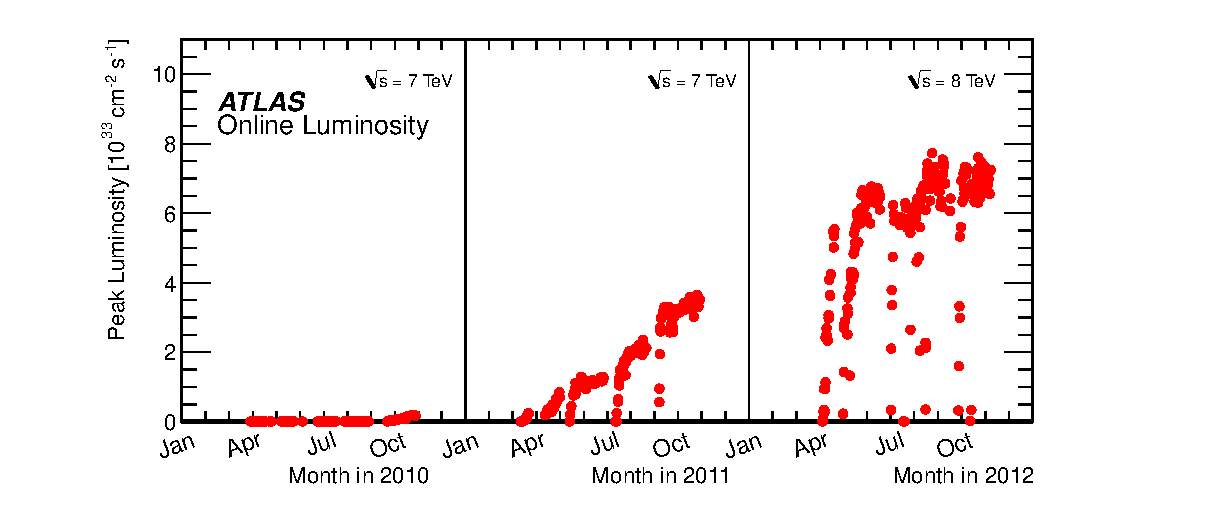
\includegraphics[width=\textwidth]{lumivstime}
%	\subfigure[]{
%            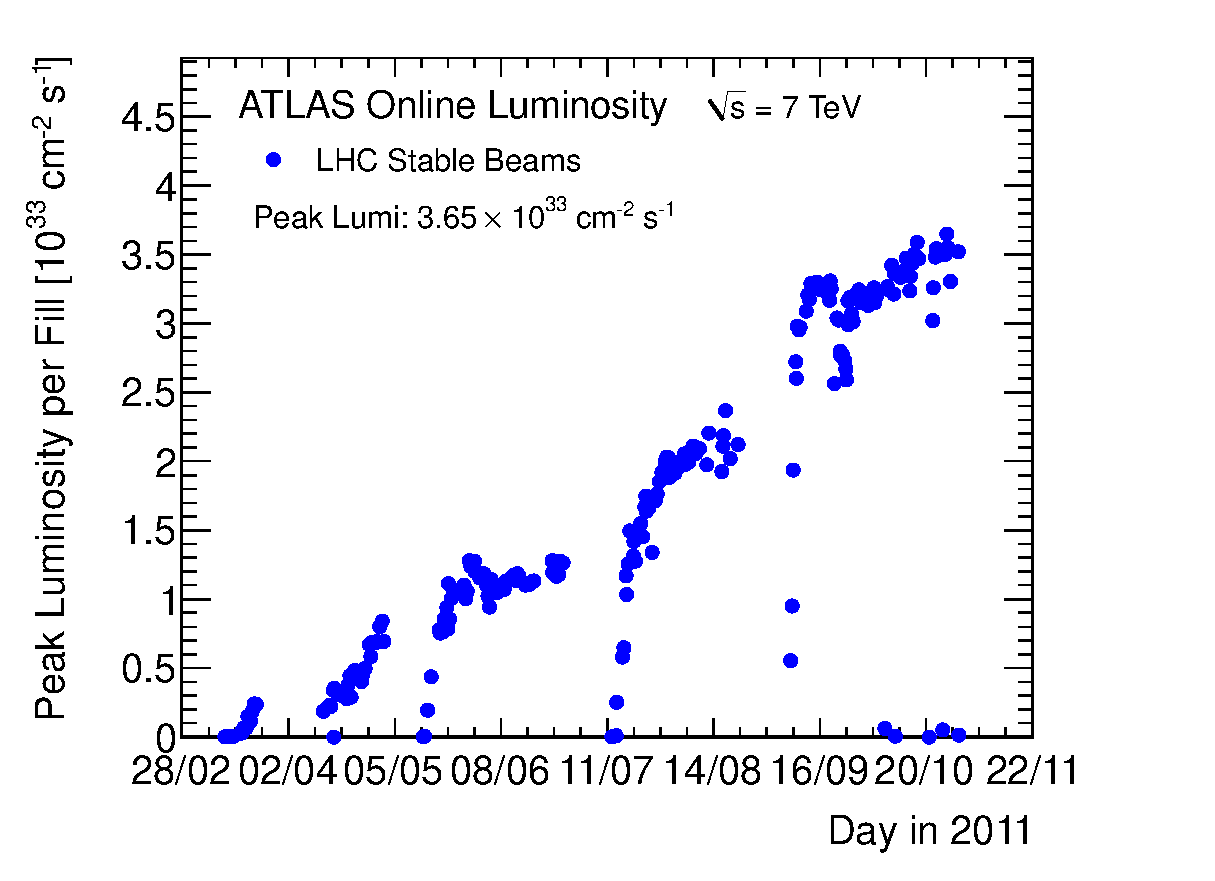
\includegraphics[width=0.47\textwidth]{peakLumiByFill2011}
%        }
%	\subfigure[]{
%            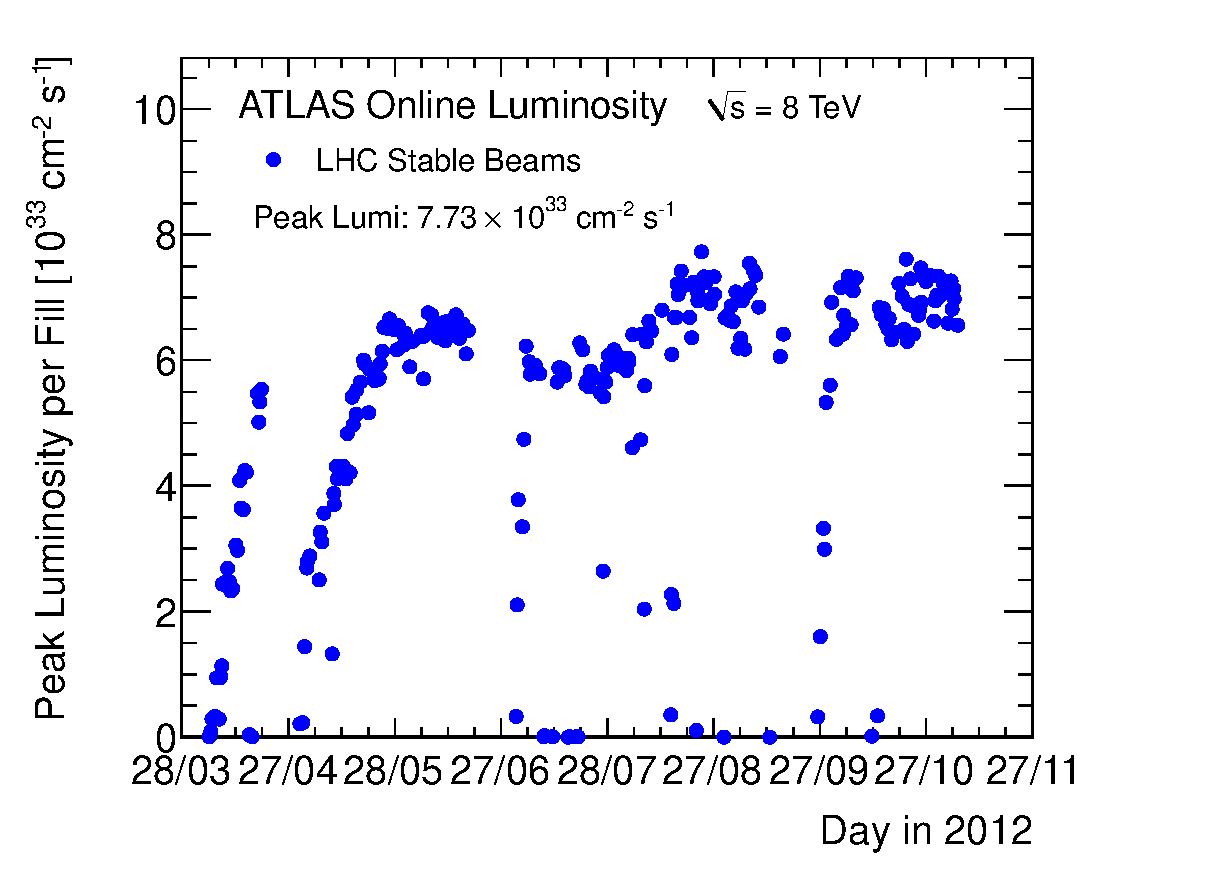
\includegraphics[width=0.47\textwidth]{peakLumiByFill2012}
%        }
\caption[Peak instantaneous luminosity delivered by the LHC per run as a function of time from
2010 to 2012.]{Peak instantaneous luminosity delivered by the LHC per run as a function of time from
2010 to 2012. Figure from~\cite{atlaslumipublic}.}
\label{fig:lhc-inst-lumi}
\end{figure}

\begin{figure}[h]
\centering
	\subfigure[]{
            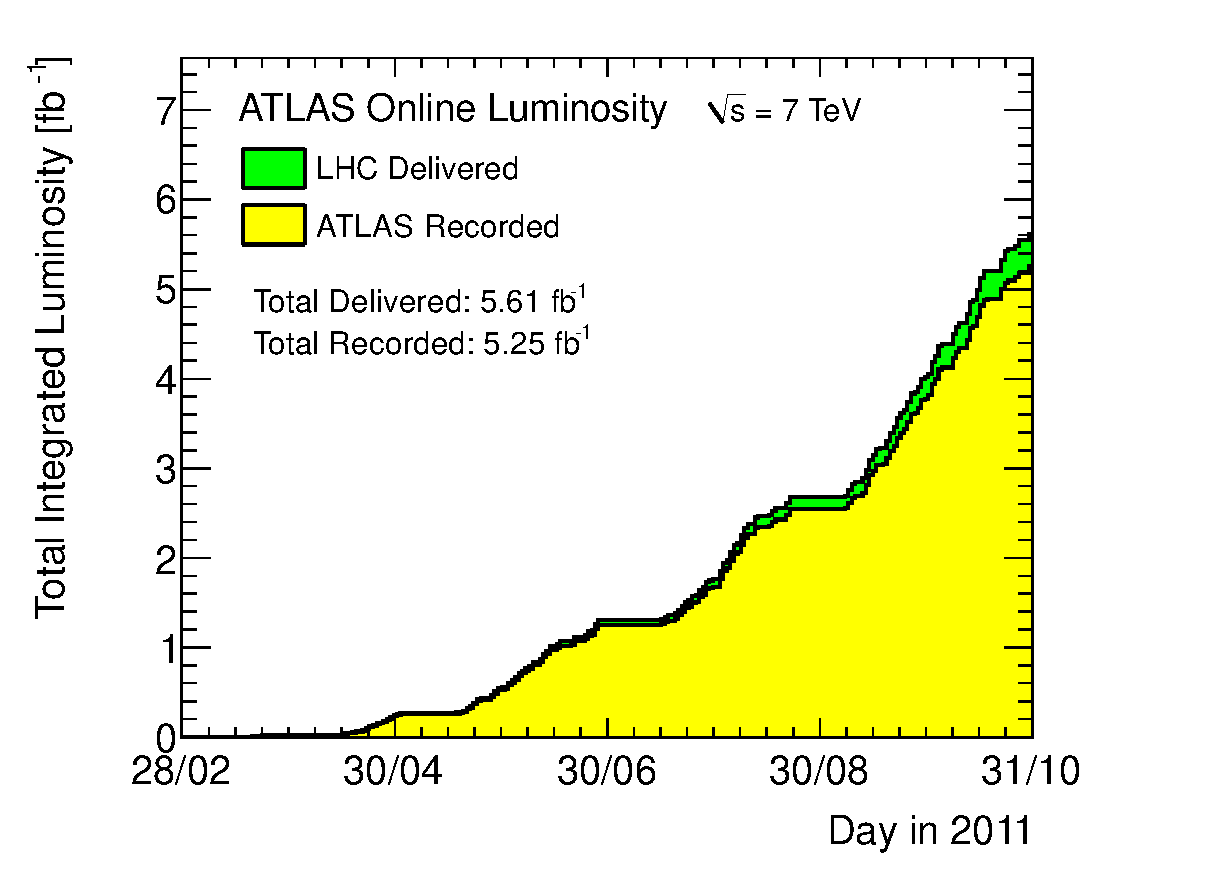
\includegraphics[width=0.47\textwidth]{sumLumiByDay2011}
        }
	\subfigure[]{
            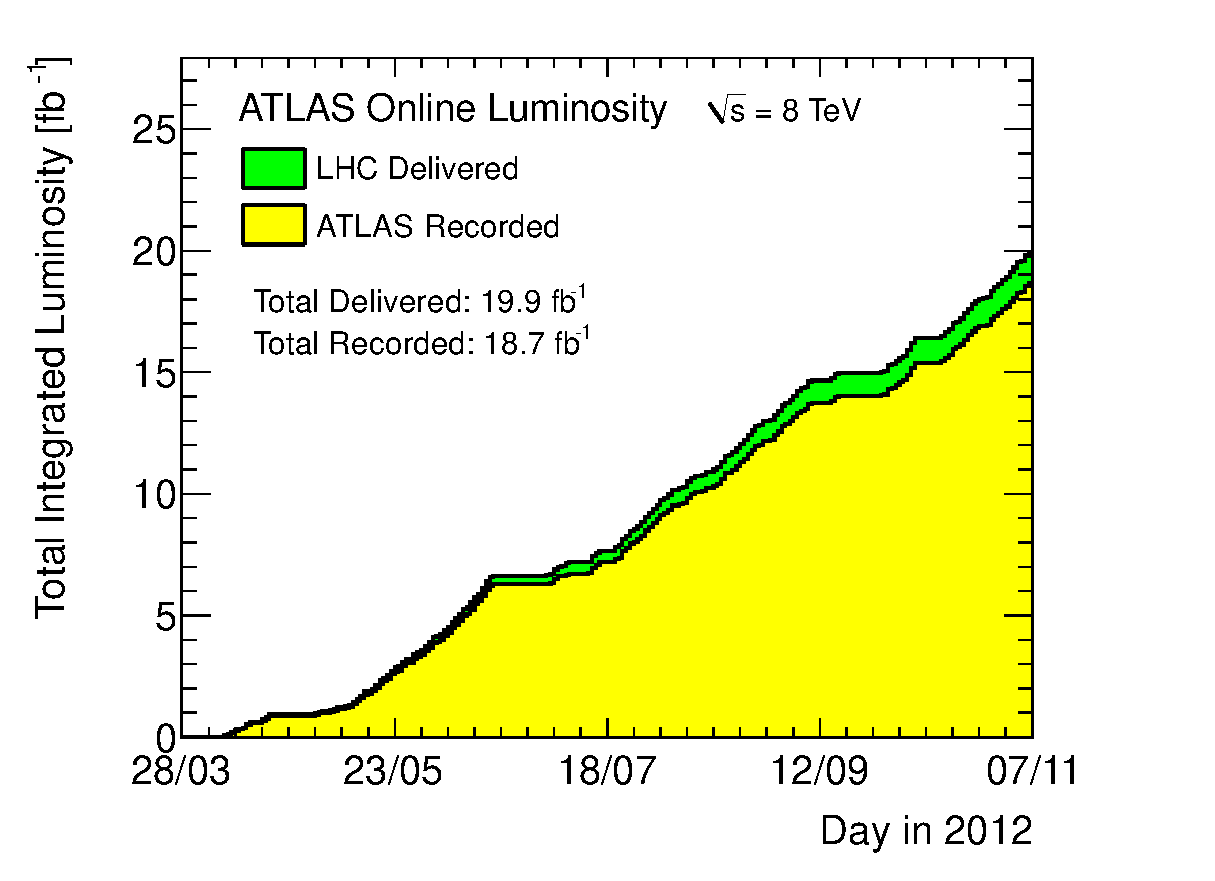
\includegraphics[width=0.47\textwidth]{sumLumiByDay2012}
        }
\caption[Cumulative integrated luminosity as a function of time in
2011 and 2012.]{Cumulative integrated luminosity as a function of time in (a)
2011 and (b) 2012. The totals for the two years are separate. 
Figures from~\cite{atlaslumipublic}.}
\label{fig:lhc-int-lumi}
\end{figure}

\fig{lhc-inst-lumi} shows the instantaneous luminosity as measured by ATLAS as a
function of time between 2010 and 2012. \fig{lhc-int-lumi} shows the cumulative
integrated luminosity delivered to ATLAS in 2011 and 2012.  Details of the LHC
operational parameters in 2011 and 2012, together with the nominal design
values, are given in~\tab{lhc-params}.

% Say something about the luminosity here
% Say something about int lumi delivered to ATLAS


% Table comparing nominal parameters, 2011, 2012
% E.g. Inst. Lumi, Bunch spacing, # bunches / beam, # protons / bunch

\begin{table}[h]
\centering
\small
\setlength{\extrarowheight}{4pt}
\begin{tabular}{ l | c | c | c  }
\hline\hline
Parameter & Nominal & 2011 Operation & 2012 Operation \\
\hline
Proton Energy & 7 \tev\ & 3.5 \tev\ & 4 \tev \\
$N_{\rm{b}}$ & 1.15 $\times~10^{11}$ & 1.5 $\times~10^{11}$ & 1.6 $\times~10^{11}$  \\
$n_{\rm{b}}$ & 2808 & 1380 & 1380 \\
Bunch spacing (ns) & 25 & 50 & 50 \\
$\beta^{*}$ (m)  & 0.55 & 1.0 & 0.6 \\
$\epsilon_{n}$ (\micro m) & 3.75 & 1.9 - 2.3 & 1.7 - 3.0  \\
Peak $\mathcal{L}$ ($\rm{cm}^{-2}\rm{s}^{-1}$) & 1.0 $\times~10^{34}$  & 3.6 $\times~10^{33}$  & 7.7 $\times~10^{33}$ \\
\hline\hline
\end{tabular}
 \caption[LHC operational parameters.]{LHC operational parameters. A comparison is made of the nominal design
 parameters~\cite{Brüning:782076}, and those used in 2011 operation and in 2012
 operation~\cite{lhcstats}~\cite{Fournier:2012np}.}
        \label{table:lhc-params}
\end{table}
% https://lhc-statistics.web.cern.ch/LHC-Statistics/

\section{The ATLAS Detector}

ATLAS (A Toroidal LHC ApparatuS) is one of two general purpose particle-physics
detectors at the LHC, built to study both proton-proton and ion-ion
interactions. The high centre of mass energy and high luminosity of LHC proton-proton collisions
allows the study of physics at the \tev\ scale for the first time, as well as
precision measurements of the Standard Model. ATLAS has been designed to be
capable of a wide range of measurements, including (but by no means limited to):
high precision tests of QCD, electroweak interactions, and flavour physics; searching for and measuring
the properties of the Higgs Boson; searches for supersymmetery; measurements
of the properties of the top quark; searches for new vector bosons and searches
for extra-dimensions. 

The extremely high luminosity presents challenges which the detector has been
designed to overcome. At design luminosity, $10^9$ inelastic collisions occur
per second, which results in multiple interactions - up to
\PeakIntPerBunchCrossing\ in 2012 running - occurring simultaneously. The
detector has been designed to cope with these high `pile-up' conditions, as well
as be capable of operating in the high radiation environment arising from the
high luminosity. Many of the physics processes of interest occur at very small
rates with respect to extremely high QCD background rates. The detector must
therefore be capable of distinguishing processes of interest from the
background. 

To meet these challenges, ATLAS was defined with the following
criteria in mind:

%In order to achieve this, ATLAS was designed to provide high granularity to cope
%with high particle fluxes and overlapping events, full azimuthal coverage to
%allow the measurement of missing transverse energy, and large coverage in
%pseudo-rapidity to provide maximum sensitivity to interesting physics processes.
%Precision tracking is required to enable good charged particle momentum
%resolution and reconstruction efficiency, and to  allow observation of secondary vertices to
%identify $b$-hadrons and $\tau$-leptons. ATLAS has precise \emag\ calorimeters
%for electron and photon identification, and full coverage hadronic calorimeters
%%for accurate jet and missing transverse energy measurement. 
\begin{itemize}
%\item Fast, radiation-hard electronics and sensors.
\item High granularity to  cope with high particle fluxes and overlapping events.
\item Full azimuthal coverage to allow for missing transverse energy
measurement, and large acceptance in pseudo-rapidity.
\item Precision tracking to provide high charged particle momentum resolution
and reconstruction efficiency, and to allow observation of secondary vertices to
identify $b$-hadrons and $\tau$-leptons.
\item Precise electromagnetic calorimetry for electron and photon
identification.
\item Full-coverage hadronic calorimetry for accurate jet and missing transverse
energy measurements.
\item High muon identification efficiency, momentum resolution and charge determination over a wide range of
momentum.
\item Efficient triggering on low transverse-momentum objects.
\end{itemize}

The main performance goals are given in~\tab{perf-goals}.

\begin{table}[h!]
\centering
\small
\setlength{\extrarowheight}{4pt}
\begin{tabular}{ l | c | c | c  }
\hline\hline
Detector Component & Design Resolution & \multicolumn{2}{| c }{$\eta$
coverage} \\
& & Measurement & Trigger \\
\hline
Tracking & $\sigma_{\pt}/\pt = 0.05\% \, \pt \oplus 1\%$ & $\pm\,2.5$ & None \\
EM Calorimetry & $\sigma_{E}/E = 10\%/\sqrt{E} \oplus 0.7\%$ & $\pm\,3.2$ &
$\pm\,2.5$ \\
Hadronic Calorimetry & & & \\
\hspace{3mm} Barrel and End-Cap & $\sigma_{E}/E = 50\%/\sqrt{E} \oplus 3\%$ &
$\pm3.2$ & $\pm\, 3.2$ \\
\hspace{3mm} Forward & $\sigma_{E}/E = 100\%/\sqrt{E} \oplus 10\%$ & $3.1<|\eta|<4.9$ & $3.1<|\eta|<4.9$ \\
Muon Spectrometer & $\sigma_{\pt}/\pt = 10\%$ at \pt\ = 1 \tev\ & $\pm\, 2.7$ &
$\pm\, 2.4$ \\
\hline\hline
\end{tabular}
 \caption[Performance goals of the ATLAS detector.]{Performance goals of the ATLAS detector. Units of \pt\ and \E\ are
 \gev.}
	\label{table:perf-goals}

\end{table}

A cut-away view of the ATLAS detector~\cite{1748-0221-3-08-S08003} is shown in~\fig{atlas-det-1}. The detector consists
of an inner tracking detector, which is
surrounded by electromagnetic and hadronic calorimeters and finally a muon
spectrometer. The \id\ is immersed in a 2 T solenoidal field to allow
for momentum measurement. The muon spectrometer is also immersed in a magnetic
field, provided by an air-core toroid system  which generates strong
bending power over a large volume with a minimum of material, thus
minimising multiple-scattering effects. A three-level trigger system is used to select events to read out.
The various sub-systems are described in more detail in the following
sections. 

\begin{figure}[h]
\centering
\includegraphics[width=\textwidth]{{lhc-pho-1998-304}.jpg}
\caption[Cut-away view of the ATLAS detector.]{Cut-away view of the ATLAS detector~\cite{Jean-Luc:841458}. The
various detector sub-systems are labelled.}
\label{fig:atlas-det-1}
\end{figure}

\subsection{ATLAS Co-ordinate System}
ATLAS uses a right-handed coordinate system with an origin at the nominal
interaction point in the centre of the detector. The \z-axis points along the
beam-pipe, the \x-axis towards the centre of the LHC ring, and the \y-axis
upwards. Particle directions and detector element positions are generally
described by their azimuthal angle $\phi$ and their pseudorapidity $\eta$. The
azimuthal angle describes the angle in the \x-\y\ plane, with $\phi=0$ along the
\x\ axis, increasing clockwise around the beam-pipe.  The pseudorapidity $\eta$
is defined in terms of the polar angle $\theta$ (the angle in the $x-z$ plane)
as $\eta = - \ln\tan(\theta/2)$, and is an approximation to rapidity in the high
energy limit.  The radial co-ordinate \R\ measures the radial distance from the
interaction point. 

\subsection{Inner Detector}

The ATLAS \id\ (ID) is located closest to the beam pipe. It is a tracking
detector designed to provide hermetic coverage and robust pattern recognition, locate
interaction vertices, including displaced secondary vertices from long-lived
particles, and provide a precise measurement of the transverse momenta of charged
particles with a nominal \pt\ threshold of 0.5 GeV. It consists
of a silicon pixel detector (the \intro{Pixel Detector}), a silicon strip
detector (the \intro{Semiconductor
Tracker} or SCT) and a transition radiation tracker (the TRT), located within a
2 T magnetic field provided by a solenoidal superconducting magnet.

\begin{figure}[h]
\centering
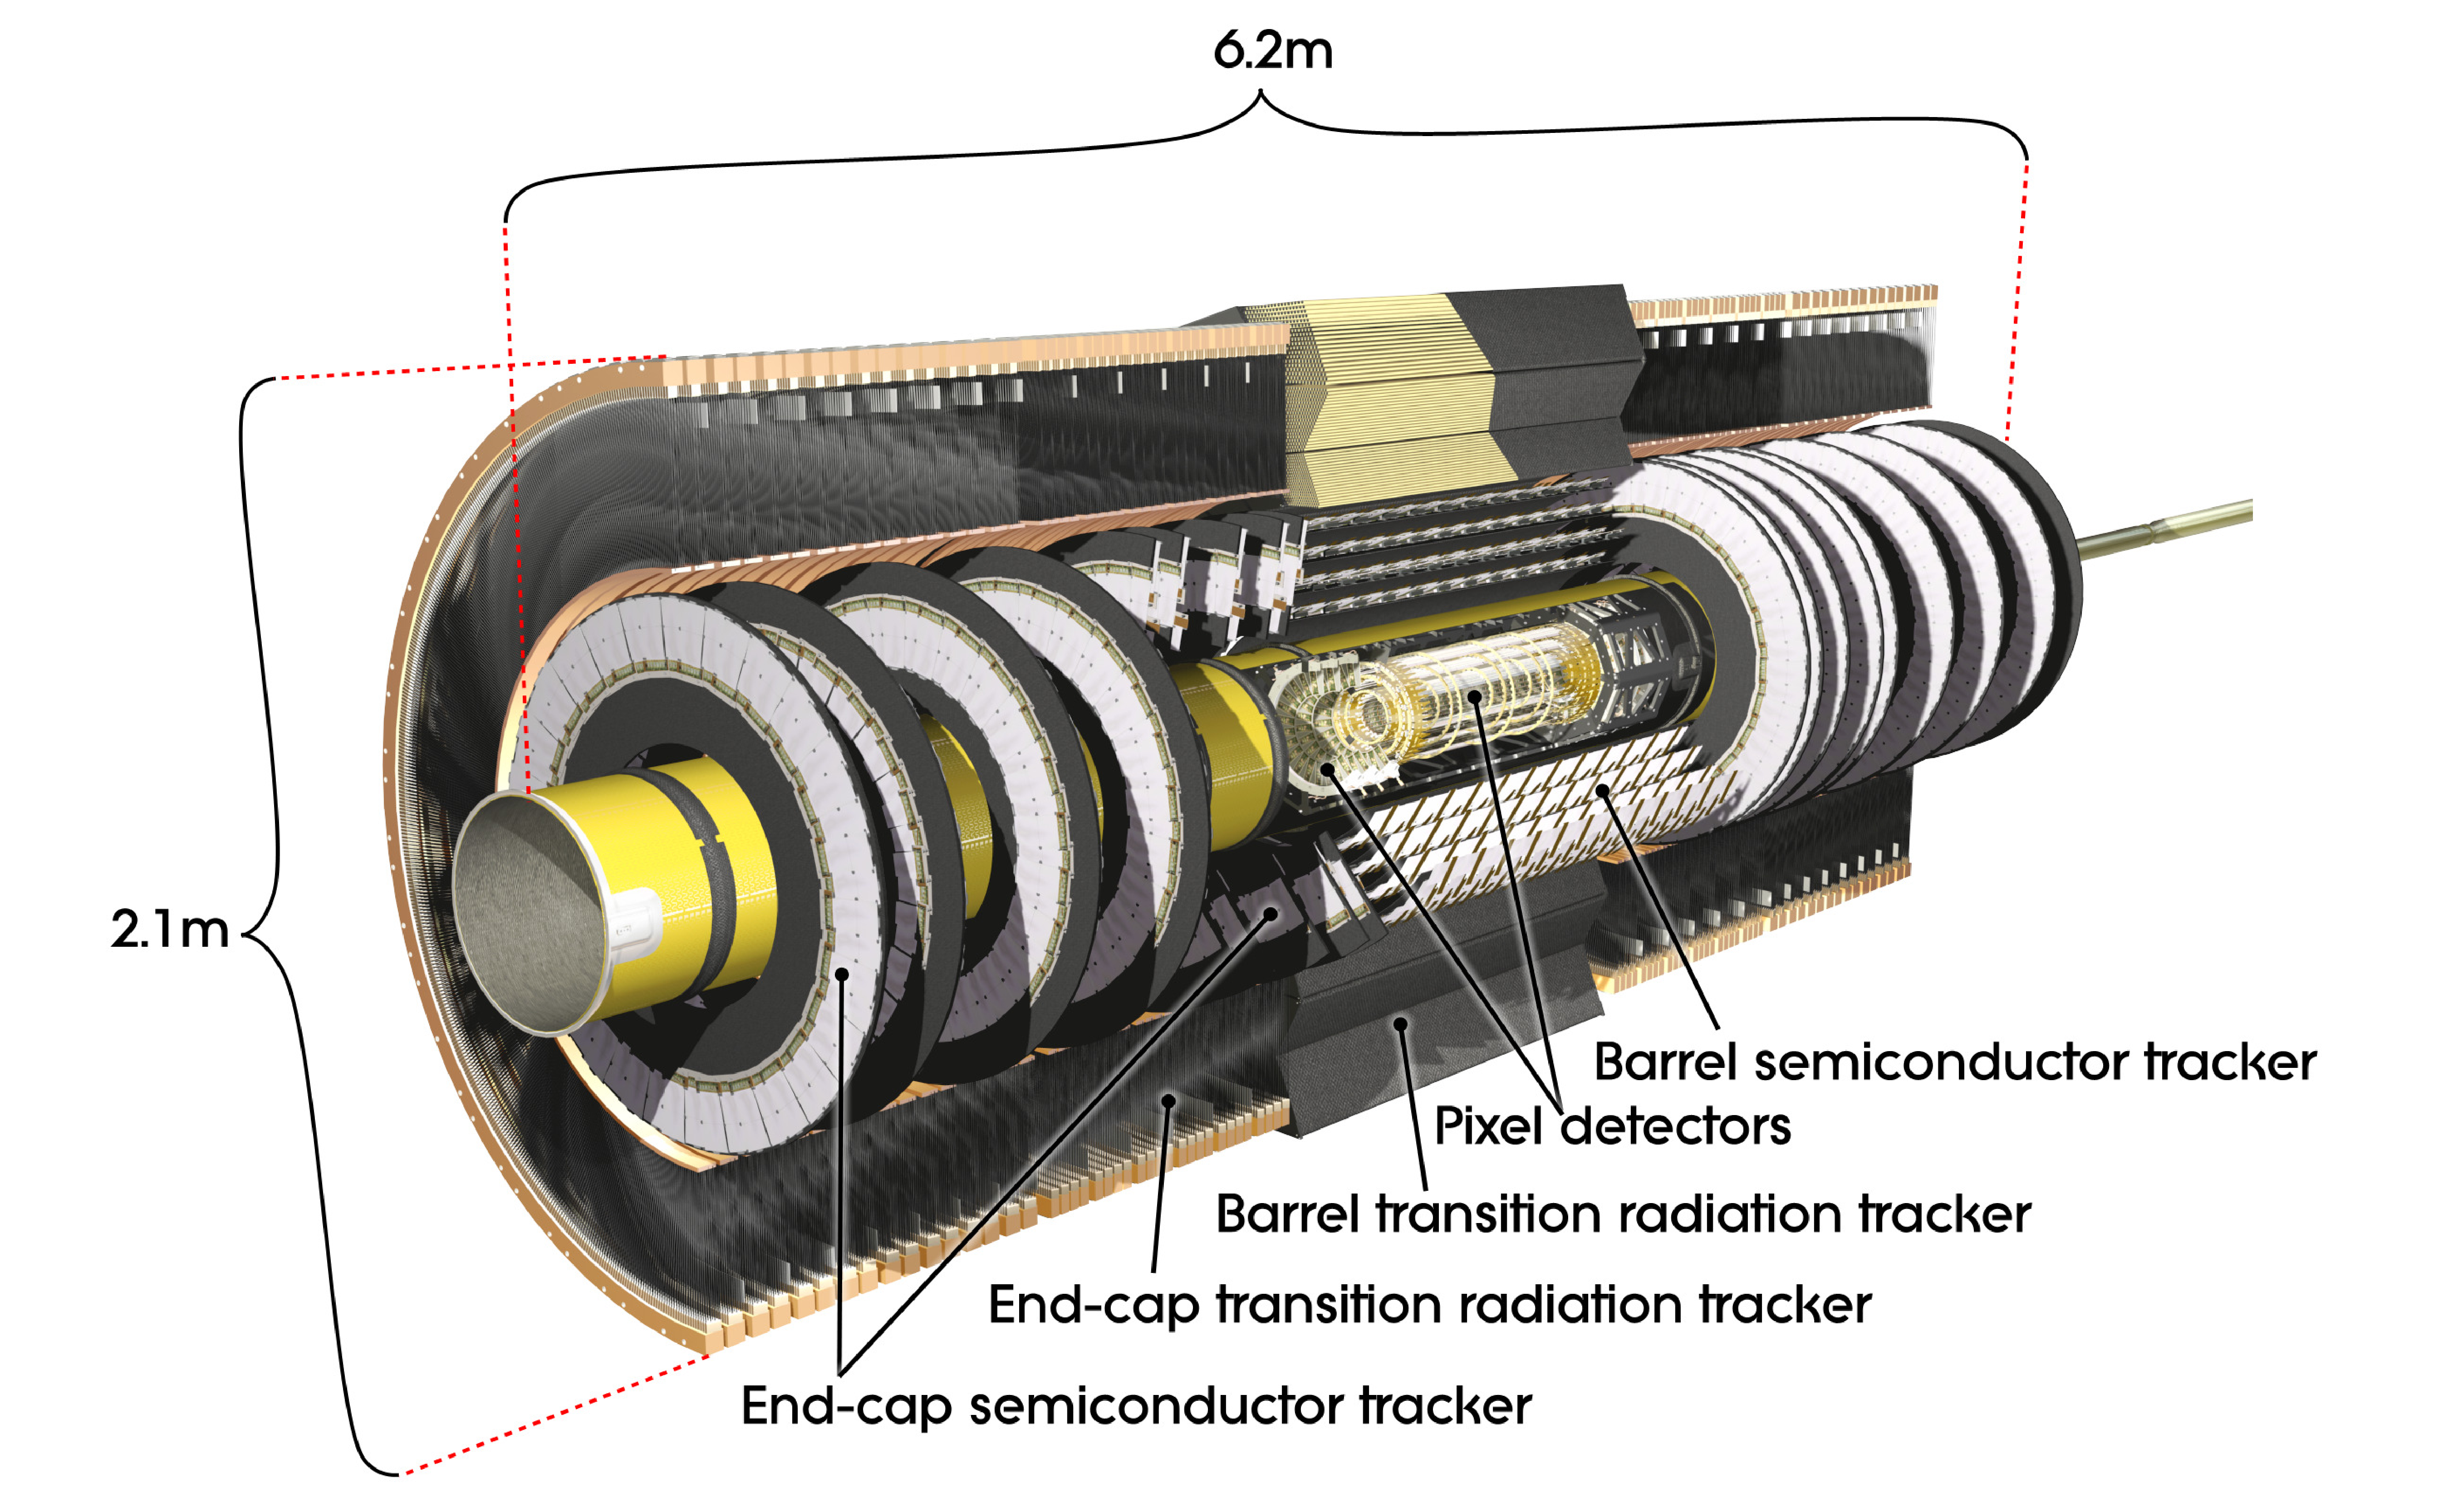
\includegraphics[width=\textwidth]{ID_newTRT_d3}
\caption[Cut-away view of the \id.]{Cut-away view of the \id, taken from~\cite{Aad:1125884}.}
\label{fig:id-1}
\end{figure}

A cut-away diagram of the \id\ is shown in \fig{id-1}. 
%The detector
%is cylindrical in shape, extending 3512 mm either side of the interaction point
%in the \z\ direction with a radius of 1150 mm. 
The subdetectors all consist of
concentric cylindrical layers surrounding the beam pipe, referred to as
`barrels', with disks referred to as `end caps' covering each end of the
barrels. A plan view of a quarter of the \id\ is shown
in~\fig{id-plan}. The Pixel and SCT detectors provide coverage for $|\eta|<2.5$,
with the TRT enhancing pattern recognition and track momentum resolution for
$|\eta|<2.0$

\begin{figure}[h]
\centering
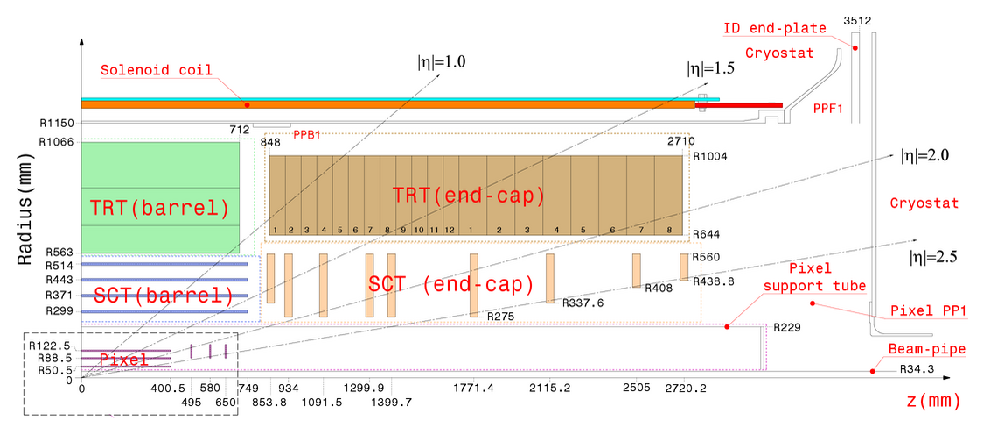
\includegraphics[width=\textwidth]{FigID26-mod-011107_crop}
\caption[Plan view of a quarter section of the \id\ showing the
positions and pseudo-rapidity coverage of the various subdetectors.]{Plan view
of a quarter section of the \id\ showing the
positions and pseudo-rapidity coverage of the various subdetectors. Figure taken from~\cite{Aad:1125884}.}
\label{fig:id-plan}
\end{figure}

\subsubsection{Pixel Detector}

The pixel detector is the detector component closest to the beam. It is formed
of layers of silicon semiconducting pixels, and is designed to have a very
high granularity for resolving primary and secondary interaction vertices. There
are three barrel layers closed by an endcap consisting of three disks at each
end. The barrels are numbered from 0 to 2. The closest layer to the beam
pipe, termed the \b-layer (due to its important role in detecting secondary
vertices for \b\ physics), is
positioned at a radius of 50.5 mm. Due to the high radiation dose that it will
receive at this position, it will need to be replaced after three years of operation at design luminosity.

% Pixels in the region of the front end chips on a module are 50x600 um^2
The detector layers are formed of silicon sensor modules, 
%of which there are 1744 in
%total. Each module consists of a 250 \micro m thick
each consisting of 46,080 active pixels with nominal dimensions of
$50\times400~\mu \rm{m}^{2}$. In total
there are approximately $80.4\times 10^{6}$ readout channels.

Particles with \modetalt{2.0} will traverse three layers of the detector; in most case
producing three space-points. The intrinsic accuracy of the position
measurement is 10 \micro m in $(\rm{R}-\phi)$ and 155 \micro m in \z\ in the
barrel layers and 10 \micro m in $(\rm{R}-\phi)$ and 155 \micro m in $\phi$ in
the endcaps.

\subsubsection{Semiconductor Tracker (SCT)}

\label{sec:Detector-SCT}

The SCT is a silicon strip detector, consisting of four barrel layers and two end-caps
consisting of nine disks each. The barrel layers consist of 2112 separate modules and
%extend from a radius of 299 mm from the beam line at the innermost layer to a
%radius of 514 mm at the outermost. The layers 
are numbered from 3 to 6. Each
endcap consists of 988 modules, arranged in such a way that a particle must pass
through four layers of the detector.

%SCT modules are made from two pairs of single sided p-in-n silicon chips biased
SCT modules are made from two layers of single sided p-in-n silicon chips biased
at 150V (this voltage will increase as the detector become radiation damaged). 
Charged particles passing through the depletion region at the centre of
the junction produce electron hole pairs, which are swept apart by the bias
voltage. The electrons are then collected on the top of the chip, producing a
signal which can be read out. A photo of an SCT barrel module is shown
in~\fig{sct-barrel-module}.

Each side of the module consists of 768 strips of length 6.4~cm,
with a pitch of 80 \micro m for barrel modules, and an average pitch of 80
\micro m for endcap modules. The strips on one layer
of the module run parallel to the
beam axis on the barrel, and along the \R\ direction on the endcap. The other
layer is placed at a stereo angle of 40~mrad to form a two-sided module. 
%give resolution in the \z\ (\R\ co-ordinate on the barrel (endcaps). 
In total
there are approximately $6.3 \times 10^{6}$ readout channels.

% From http://atlas.web.cern.ch/Atlas/GROUPS/INNER_DETECTOR/SCT/gallery/barrel_modules/barrelmodule.jpg
% but could cite detector paper if need be
\begin{figure}[h]
\centering
\includegraphics[width=0.8\textwidth]{{SCTbarrelmodule}.jpg}
\caption[Photograph of an SCT barrel module.]
{Photograph of an SCT barrel module. Figure
from~\cite{1748-0221-3-08-S08003}}
\label{fig:sct-barrel-module}
\end{figure}

%Each pair of chips is wire-bonded together and two
%pairs 
 The readout is of a binary form, with a charge collection threshold of 1
fC (chosen to maximise efficiency and minimise noise). To form a space-point, a
coincidence of hits on either side of the module is required. The stereo
angle gives the ability to determine where along the strip the hit occurred,
giving resolution in \z\ (\R) in the barrels (endcaps). A small angle is used to
prevent ambiguities in the presence of multiple nearby hits (so called `ghost
hits'). The spatial
resolution of the detector is 17~\micro m in ($\rm{R}-\phi$) and 580~\micro m in
\z\ (\R) in the barrel (endcaps).

\subsubsection{Transition Radiation Tracker (TRT)}
\label{sec:Detector-TRT}

The Transition Radiation Tracker is a straw drift tube tracker, with additional
particle identification capabilities from transition radiation. It consists of
modules formed from bundles of 4 mm diameter straws, filled with
$\rm{XeCO_{2}O_{2}}$ gas. A tungsten wire 
%of 30 \micro m diameter 
runs down the centre of the tube to collect charge. In the barrel the straws run
parallel with the beam axis and 
%are 144 cm long. The wires 
are electrically divided into two halves at \modetaeq{0} and read out at either
end (this subdivision leads to an inefficiency along a length of approximately 2
cm at the centre of the TRT). In the endcaps the straws 
%are 37 cm long and 
run radially. In total there are 351,000 readout channels.

% Number of hits - resolution - advantages of continuous tracking
All charged tracks with \ptgt{0.5} and \modetalt{2.0} will traverse at least 36
straws, except in the barrel to endcap transition region (\modetabetween{0.8}{1.0})
where only 22 straws will be traversed. The ($R-\phi$) resolution is 130 \micro
m. Despite the low resolution compared to the silicon trackers, and the lack of
a measurement in the \z\ direction, the hits in the TRT contribute significantly
to the pattern recognition and momentum resolution due to the large number of
measurements and longer measured track length.

% TR
The barrel straws are embedded in a matrix of 
%19 \micro m diameter 
polypropylene fibres, and the endcap disk layers are sandwiched between 
%15 \micro m
polypropylene foils. When charged particles cross the boundary between the straw
and the fibre they emit transition radiation photons. These photons are then
absorbed by the Xenon gas mixture, and produce much larger signals than
minimum-ionising charged particles. The energy of the transition radiation
photons depends heavily on particle type, and is approximately 200 keV for a 20
GeV electron and 1 keV for a 20 GeV pion. This difference can be exploited for
particle identification, by counting the number of hits over a higher energy threshold.
Electrons with \ptgt{2} typically produce 7 - 10 high threshold hits, whereas
pions and other charged particles will produce far fewer.

\subsection{Calorimetry}

The ATLAS
calorimeter systems sit outside the \id\ and its magnetic field. 
The purpose of the calorimeter is to measure the energy and
position of particles. A particle entering the calorimeter produces a
`shower' of secondary particles; the energy of this shower is then measured.
ATLAS uses sampling calorimeters, in which different materials sandwiched
together in layers, are used to initiate the shower development (absorption) and
to measure the energy of its constituents. This
allows for a more compact design and hence better shower containment. Position
measurement is obtained by segmenting the calorimeter in the \z\ and $\phi$
directions.

Different absorbers are required depending on whether the particle interacts
via the electromagnetic or the strong force, and the properties of the showers that develop
are different. The ATLAS calorimeters are divided into two distinct subsystems,
the \emag\ calorimeter and the hadronic calorimeter. An electromagnetic
shower consists of electrons and photons, and is normally fully contained in the
calorimeter; thus it can be fully detected. Hadronic showers involve many more
particles types, including neutrons, muons, and neutrinos which escape detection, and tend
to be longer and wider, often spilling out of the calorimeter. The full energy
of the shower is thus not fully detected, and so a calibration of the energy
response is required. It is important for the calorimeter to provide good
containment of electromagnetic and hadronic showers, not only for the purposes
of energy measurement, but also to allow a good missing transverse energy
requirement, and to prevent punch-through into the muon system.

\begin{figure}[h]
\centering
\includegraphics[width=0.9\textwidth]{{0803015_01}.jpg}
\caption[Cut-away view of the ATLAS calorimeter system.]{Cut-away view of the ATLAS calorimeter system. Image taken
from~\cite{1748-0221-3-08-S08003}.}
\label{fig:calo-cutaway}
\end{figure}

A cutaway view showing the location of the various calorimeter elements is shown
in~\fig{calo-cutaway}. The calorimeters cover the range \modetalt{4.9}. Over the
$\eta$ range of the inner-detector, the \emag\ calorimeter gives fine
granularity to allow precise measurement of electrons and photons. The hadronic
calorimeter is more coarsely segmented, but is sufficient to meet the
requirements of jet and missing transverse energy measurement.

\subsubsection{Electromagnetic Calorimeters}

The \emag\ (EM) calorimeter 
(also referred to as the \intro{LAr}) 
uses liquid
argon as the active detector material, and lead as an absorber. 
%Incident
%particles ionise atoms in the lead absorber, creating an electromagnetic shower.
Charged particles in the shower ionise the liquid argon, where the electrons
drift to copper electrodes in the presence of an electric field.

The LAr consists of two half barrels extending to \modetalt{1.475} (with
a 4~mm gap at \z\ = 0), and two coaxial wheels on each side (named the
\intro{EMEC}, the first covering
\modetabetween{1.375}{2.5} and the second covering \modetabetween{2.5}{3.2}.
Additional material needed to instrument and cool the detector creates a `crack'
region at \modetabetween{1.375}{1.52}, where the energy resolution is
significantly degraded.

The barrel calorimeter has an accordion structure in order to avoid azimuthal
cracks and to provide full $\phi$ symmetry, as shown in~\fig{lar-diagram}. The
accordion structure is made of the lead absorber, with the liquid argon filling
the 2.11 mm gaps between the absorbers. The barrel of the LAr calorimeter is
divided into three layers, with different cell granularity. The first layer is
divided into cells of \deltaetadeltaphi{0.0031}{0.098}. The fine granularity in
$\eta$ of this layer is used to determine the pseudo-rapidity of the particle,
and for measurements of the shower shape, an important input to particle
identification. The second layer has cell size \deltaetadeltaphi{0.0245}{0.025}
and contains the largest energy fraction of the shower, measuring approximately
16 radiation lengths. The third layer, with cell size
\deltaetadeltaphi{0.0245}{0.05}, collects the tail of the shower. The first
wheel of the LAr calorimeter is also segmented into three layers with the same
granularity as the barrel. The second wheel has a coarser granularity that
varies as a function of pseudorapidity. A liquid argon pre-sampler exists for
\modetalt{1.8} to correct for energy lost by incident particles traversing
material before the calorimeters, and to aid with discriminating between
$\pizero \to \gamma \gamma$ decays and prompt photons.

%The liquid argon has to be maintained at a temperature of 88 K.

\begin{figure}[h]
\centering
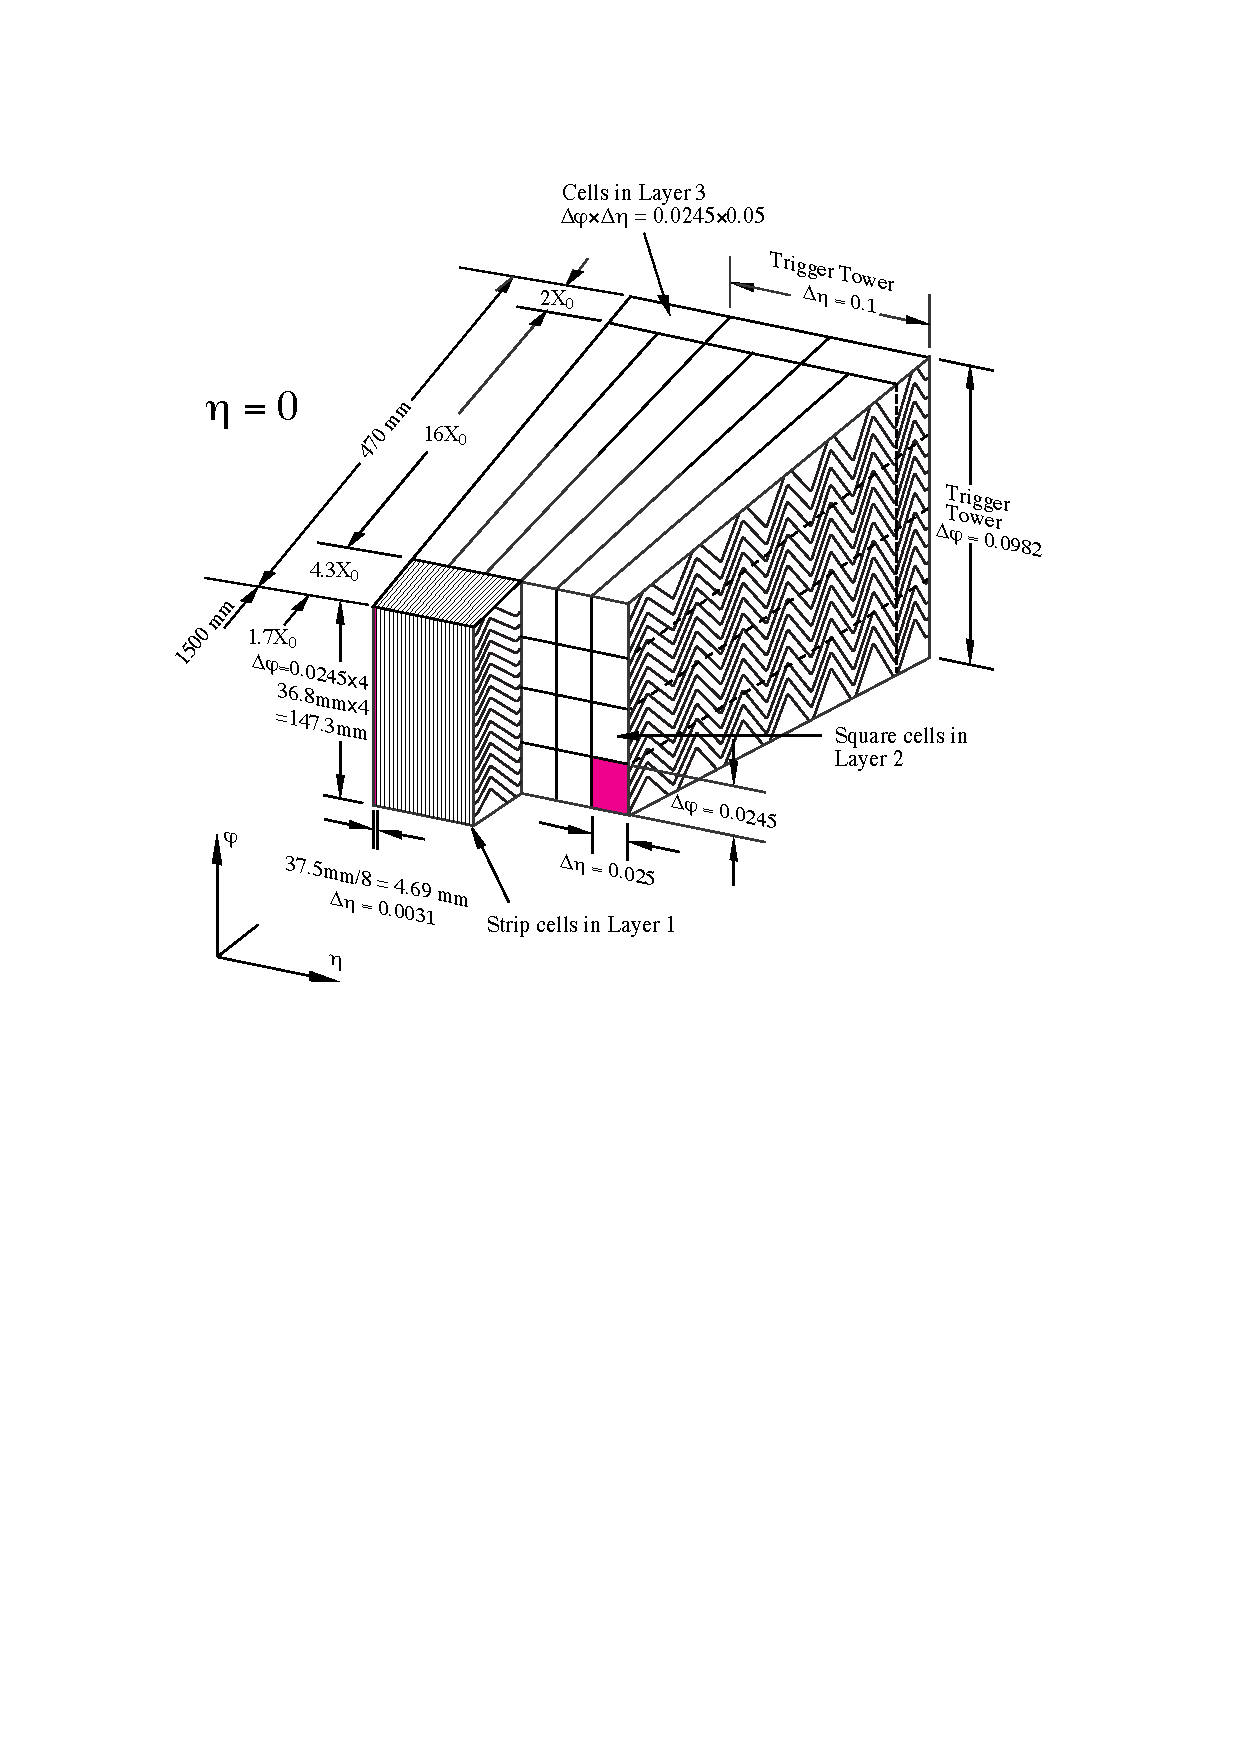
\includegraphics[width=0.8\textwidth]{lar-diagram}
\caption[Diagram of the ATLAS liquid argon calorimeter, showing the accordion
structure and the different granularity in the different layers.]{Diagram of the ATLAS liquid argon calorimeter, showing the accordion
structure and the different granularity in the different layers. Diagram taken
from~\cite{1748-0221-3-08-S08003}.}
\label{fig:lar-diagram}
\end{figure}

\subsubsection{Hadronic Calorimeters}

The hadronic calorimeter consists of a plastic scintillator tile calorimeter 
(referred to as the \intro{tile} calorimeter) covering \modetalt{1.7} and a liquid
argon endcap calorimeter (referred to as the \intro{HEC}) covering
\modetabetween{1.5}{3.2}. 

The tile calorimeter consists of a 
%5.8 m long 
barrel covering \modetalt{0.8} and two 
%2.6~m long 
extended barrels covering \modetabetween{0.8}{1.7}, and is located immediately
behind the EM calorimeter. 
%extending from a radius of 2.28 m~to a radius of 4.25~m. 
The active material consists of 3~mm thick layers of the plastic scintillator
placed perpendicular to the beam direction, sandwiched between steel absorbers.
The scintillators are connected at each end to readout photomultiplier tubes by
wavelength-shifting fibres. The fibres are grouped together to form readout
cells, giving projective towers in $\eta$. There are three layers of cells, with
a granularity of \deltaetadeltaphi{0.1}{0.1} in the first two layers, and
\deltaetadeltaphi{0.1}{0.2} in the third.

The HEC consists of two wheels per endcap, HEC1 and HEC2, located directly
behind the EMEC and sharing the same cryostat. Each wheel has two layers of
cells. The HEC covers \modetabetween{1.5}{3.2} and so overlaps with the tile
calorimeter on one side and the FCAL on the other, thus avoiding cracks in the
transition regions. HEC1 (HEC2) is built from 25 mm (50 mm) copper plate
absorbers interleaved with 8.5 mm gaps containing liquid argon. The liquid
argon gaps are split into four drift spaces of roughly 1.8 mm by three
electrodes. This is to avoid ion build-up due to the higher particles fluxes
and energies in the forward region, and also allows a lower high voltage than a single
electrode design.

\subsection{Forward Calorimeter}

The forward calorimeter ({\it FCAL}) covers \modetabetween{3.1}{4.9}. To reduce the
neutron flux, the FCAL begins 1.2 m away from the EM calorimeter
front face. Due to the high particle fluxes and energies in the forward region,
the calorimeter must contain relatively long showers in the small volume allowed
by design constraints, and thus must be very dense. The FCAL is divided into
three compartments. The first, FCAL1, is designed for electromagnetic
measurements, and uses copper as an active material with liquid argon as a
passive material. The second two compartments, FCAL2 and FCAL3, are designed for hadronic
measurements, and use tungsten as a passive material, chosen for its high
density to provide containment and minimise the lateral spread of hadronic
showers. An additional copper alloy shielding plate is placed behind FCAL3 to
reduce background to the muon endcap system.

\subsection{Muon Spectrometer (MS)}

The muon spectrometer sits outside the calorimeter system, and is designed to
provide precision muon momentum measurements over a momentum range of 3~GeV to
3~TeV, as well as providing triggering on bunch crossings containing
muons. An overview of the MS is given in~\fig{muon-cutaway}. The system sits
inside a giant air coil toroidal magnet system, producing a magnetic field
orthogonal to the muon momentum to provide deflection of the
muons for momentum measurement. The use of an air coil reduces multiple
scattering which degrades the momentum resolution.

\begin{figure}[h]
\centering
\includegraphics[width=0.8\textwidth]{{ms_cutaway}.jpg}
\caption[Cut away view showing the various components of the ATLAS muon
spectrometer.]{Cut away view showing the various components of the ATLAS muon
spectrometer. Figure taken
from~\cite{1748-0221-3-08-S08003}.}
\label{fig:muon-cutaway}
\end{figure}

Resistive Plate Chambers (RPC) and Thin Gap Chambers (TGC) provide triggering
for \modetalt{2.4} and a measurement in the $x-y$ plane for \modetalt{2.7}. The
RPC covers \modetalt{1.05}, with the TGC covering \modetabetween{1.05}{2.7}. The
muon trigger has a time resolution of between 1.5 ns and 4 ns.

Precision measurements in the bending ($R-z$) plane are obtained from Monitored
Drift Tubes (MDT) and Cathode Strip Chambers (CSC). The MDT cover \modetalt{2.7}
and consists of three layers, referred to as \intro{stations}. Each station
consists of two \intro{mulitlayers} formed of three of four layers of tubes,
sandwiched between layers of RPC or TGC.
%The mechanical isolation of the sensor wire in each tube from it's neighbours
%give a reliable system design.
In the innermost layer, for \modetabetween{2.0}{2.7} the MDT are replaced by CSC
due to the higher rates and higher backgrounds in this region. The CSC are
multiwire proportional chambers, and so give a higher granularity than the MDT,
and are better able to cope with high rates and fluxes. 

\section{Trigger}
\label{sec:detector-trigger}

ATLAS uses a three-level trigger system to identify when to read out the
detector and to reduce the event rate to a manageable level by identifying
interesting events. The collision rate of approximately 20 MHz has to be reduced
to a rate of between 200 and 1000 Hz for offline reconstruction, storage and analysis.
An overview of the ATLAS trigger system is shown in~\fig{trigger_overview}. 

The
first level, L1, uses fast custom electronics to identify the presence of signals from a hard scattering such as
high \pt\ electrons, muons or jets, or a large amount or missing transverse
energy. The L1 trigger has a maximum latency of 2.5 \micro s, and must reduce
the rate to approximately 60 kHz (the design L1 rate was 75 kHz, however
significant detector dead-time has been observed above 65 kHz). To meet this
tight time constraint, only low-granularity signals from the calorimeters and dedicated muon trigger
chambers are used. The L1 trigger also identifies `Regions of Interest' (RoI)
surrounding the signature that caused the trigger to be fired, for use in later
levels of the trigger.

The second (L2) and third level (the \intro{Event Filter} or EF) trigger are software based, and are collectively known as the
`High Level Trigger' (HLT). At each level, the decision of the previous level is
refined by using more detector information and allowing a longer time for the
decision to be made and thus more complicated algorithms to be run, as well as
tightening the selection requirements to further reduce the rate. At L2 the full
readout from the RoIs identified at L1 is available. L2 uses dedicated
algorithms to return a decision based on the RoI information within 100 ms. The
EF has access to the full event readout, although typically only information
inside or just outside the RoI is used. The EF algorithms are based on the
offline object reconstruction algorithms, and may take up to 1~s to make
a decision.

The trigger is organised into `chains' with an L1 trigger seeding a chain of
algorithms in the HLT. Each chain is responsible for selecting a specific
trigger signature. The `trigger menu' is the collection of chains used to select
data during a run. It typically consists of about 200 primary chains for selecting data
for physics analysis and about 300 supporting chains for selecting data for
background and performance studies. The design of the trigger menu involves
balancing between the sensitivity for physics analysis resulting from the
trigger, and the need to reduce the rate to a level dictated by the available
resources for reconstruction and storage. The offline computing processing power
limits the EF trigger rate to about 400 Hz. The trigger menu had to evolve
throughout 2011 and 2012 to meet challenges posed by the constant increase in
instantaneous luminosity, and the increase of pileup to almost double the design
value. The measurements described in this thesis use single electron and muon
triggers. These triggers account for the largest slice of the trigger bandwidth,
with rates of approximately 50 Hz each. They are described in more detail
in Sections~\ref{sec:reco-el-triggers} and \ref{sec:reco-mu-triggers}.

\begin{figure}[h]
\centering
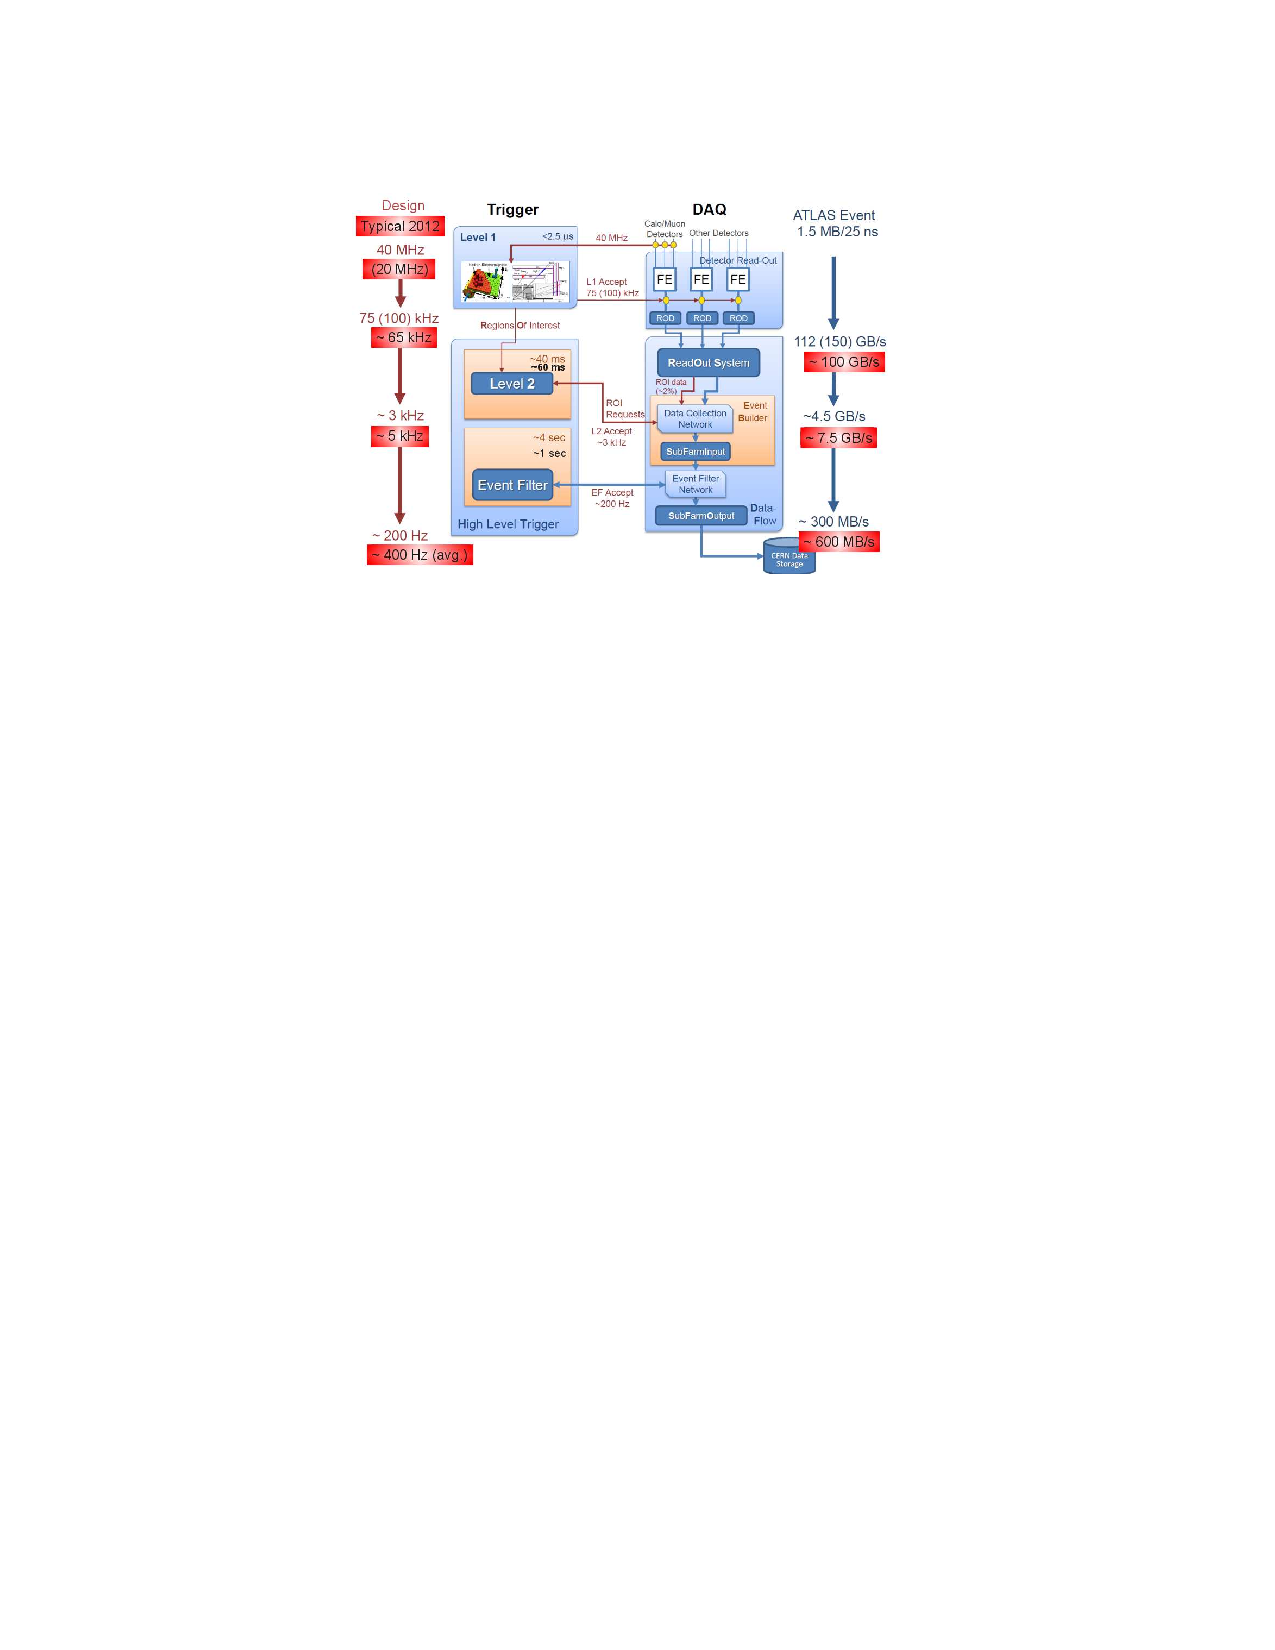
\includegraphics[width=0.8\textwidth]{trigger_overview}
\caption[An overview of the ATLAS trigger and DAQ system.]{An overview of the ATLAS trigger and DAQ system. The design and 2012
typical trigger rates at each level are shown on the left, and the design and
2012 typical output bandwidths are shown on the right. Figure taken
from~\cite{Petersen:1491585}.}
\label{fig:trigger_overview}
\end{figure}

\section{Detector Simulation}

Simulation of the detector response to various physics processes is a vital
ingredient to making a physics measurement. It is important for understanding and
calibrating the detector response to different signatures, for estimation of
acceptances and efficiencies, and also to be able to compare experimental
results with theoretical models. A custom detector simulator, which uses the
\geant~\cite{Agostinelli2003250} toolkit, is used to simulate interactions
between particles and matter in the ATLAS detector. It takes as input the output
of Monte-Carlo generators as described in~\sec{Theory-MC} in HepMC format, with all
particles with a lifetime less than $c \tau > 10$ mm decayed by the generator.
The simulator then propagates the particles through the ATLAS detector, using
\geant\ to simulate their interaction with the material of the detector. 

The response of the detector components to the particles produced is also
simulated, and simulated output signals are produced in the same format as the
real detector output. These are then reconstructed in the same way as for real
data (as described in~\chap{Reconstruction}). To simulate the effect of pileup,
minimum bias events generated with the \pythia generator are overlaid with the
hard event.

\section{Luminosity Measurement}

An accurate measurement of the delivered luminosity is an essential ingredient
to any physics analysis, for example to enable the measurement of a \cx\ or to
allow the correct normalisation of simulated backgrounds. The instantaneous
luminosity can be expressed as:
\begin{equation}
\mathcal{L} = \frac{ \mu n_{\mathrm b} f_{\mathrm r} }{ \sigmaInel }
\label{eqn:lumi-meas-1}
\end{equation}
where $\mu$ is the number of interactions per bunch crossing, $n_{\mathrm b}$ is the
number of colliding bunch pairs, $f_{\mathrm r}$ is the bunch crossing frequency, and
\sigmaInel\ is the inelastic \cx. The
instantaneous luminosity is measured during data taking by measuring the
observed interaction rate per bunch crossing \muVis~\cite{ATLAS-CONF-2011-116,Aad:2011dr}. \eqn{lumi-meas-1} can
be rewritten in term of this quantity:
\begin{equation}
\mathcal{L} = \frac{ \muVis n_{\mathrm b} f_{\mathrm r} }{ \sigmaVis }
\label{eqn:lumi-meas-2}
\end{equation}
where $\sigmaVis =\epsilon \sigmaInel$ is the total inelastic \cx\
multiplied by the efficiency of the method used to measure \muVis. The
parameters $\mu_{\mathrm{b}}$ and $f_{\mathrm{r}}$ are known machine parameters, and so a
measurement of \muVis\ gives a measurement of the relative luminosity; this
must be calibrated by measuring \sigmaVis\ in order to give an absolute
luminosity measurement.

Two primary detectors are used for the measurement of \muVis:
LUCID~\cite{Villa:1222513} and the BCM~\cite{1748-0221-3-02-P02004}.  LUCID is
specifically designed for measuring the luminosity delivered to ATLAS, and is a
Cerenkov detector consisting of sixteen aluminium tubes filled with
$C_{4}F_{10}$ gas, surrounding the beampipe each side of the interaction point
at a distance of 17 m. The Cerenkov photons are reflected down the tubes to
photomultipliers (PMTs); if one of the PMTs records a signal over threshold the
tube records a `hit' for that event. LUCID receives signals directly from the
LHC clock, allowing it to record event rates separately for each bunch crossing,
and is separate from the main ATLAS DAQ enabling luminosity measurement even
when the detector is not in data-taking mode. The BCM (Beam Conditions Monitor)
is primarily designed to measure beam-induced backgrounds and issue a beam-abort
request in case of dangerous levels of background that would be damaging to
ATLAS. It consists of four diamond sensors located on each side of the
interaction point at a distance of 1.8 m; diamond sensors are chosen for their
radiation hardness and fast readout. The fast readout means it also provides a
bunch-by-bunch signal which can be used as a measure of \muVis. Since
the efficiencies of the BCM and LUCID are different, they will measure a different
\muVis\ and hence need to be calibrated separately.

The calibration of \sigmaVis\ is done using dedicated \intro{van Der Meer (vdM)
scans}, where the absolute luminosity is measured directly from machine
parameters. The delivered luminosity can be written as:
\begin{equation}
\mathcal{L} = \frac{ n_{\mathrm{b}} f_{r} n_{1} n_{2}}{ 2 \pi \Sigma_{x} \Sigma_{y} }
\label{eqn:lumi-meas-3}
\end{equation}
where $n_{1},n_{2}$ are the bunch charges in each beam, and
$\Sigma_{x},\Sigma_{y}$ are the vertical and horizontal width of the beam. In
a vdM scan, the beams are separated in steps of known distance, and the change
in event rates measured. From this the beam widths 
$\Sigma_{x},\Sigma_{y}$ can be deduced. The bunch charge product $n_{1}\cdot
n_{2}$ is measured by two DC
current transformers, which have high accuracy but are unable to resolve
individual bunch charges, and two fast beam current transformers (FBCT) which
have lower accuracy but are able to resolve each
bunch~\cite{lhc-beam-currents}. 
Combining these two measurements, a direct measurement of the luminosity is made. By
comparing the peak luminosity (when the beam separation is at a minimum) with
the peak interaction rate measured by LUCID or the BCM, and using Equations~\ref{eqn:lumi-meas-2}
and~\ref{eqn:lumi-meas-3}, a measurement of \sigmaVis\ is obtained, enabling
absolute normalisation of the luminosity.

The luminosity measurement is \crosscheck ed using an independent measurement of
the luminosity using information from the ATLAS calorimeters. The PMT current
from the tile calorimeter and the total ionisation current in the liquid argon
of the FCal are related to the mean number of particles interaction in the
calorimeter, and so are sensitive to the luminosity. 
%The stability of the
%luminosity measurement over longer periods is cross-checked using the number of
%\Z\ bosons observed in a given period of running. 

\section{Data Samples}

The measurements described in this thesis use data collected in 2011 and 2012,
and correspond to the full proton-proton datasets collected by ATLAS in each of those two
years. The dataset is broken down into {\it runs}, continuous periods of
data-taking typically corresponding to one fill of the LHC. Each run is further
broken down into {\it luminosity blocks} consisting of roughly two or three
minutes-worth of data-taking. Runs are grouped together into {\it periods}, with
the accelerator, detector and trigger conditions being similar in each period.
The periods within each year are labelled A to M.

Luminosity blocks where there were problems with the detector (for example a HV
trip in the LAr) which would affect the reconstruction of electrons, muons, jets
or other physics objects are removed using a ``Good Runs List'' which records
which luminosity blocks have such defects. After removing these luminosity
blocks the integrated luminosity of 2011 dataset is
\LumiPassGRLTwentyEleven~\ifb\
and the integrated luminosity of the 2012 dataset is
\LumiPassGRLTwentyTwelve~\ifb. The uncertainty on the luminosity measurement is
\LumiUncTwentyEleven\ for 2011 data and
\LumiUncTwentyTwelve\ for 2012 data.

% Performance of the detector over these periods ?
